\chapter{Results}
In the following the evaluation results of the VL53L0X sensor and of the whole avoidance system are presented. 
\section{VL53L0X}
\label{sec:vl53l0x}
By evaluating the VL53L0X sensor we wanted to prove its ability for autonomous obstacle avoidance. First, we analysed the sensor on its ability to accurately measure the distance to different surfaces without a IR source (\crefrange{fig:surface_hist_con}{fig:surface_hist_white}). We conducted 100 measurements per surface at a distance of \unit[200]{mm}. We compared a white plastered, a concrete and a wooden wall. No significant difference between the surfaces can be observed. All data shows a Gaussian distribution. The deviation from the ground truth distance can be explained with measurement errors of the ground truth distance. Next, we varied the angles of the sensor relative to the wall at a constant distance of \unit[200]{mm}. (\crefrange{fig:angle90}{fig:angle22.5}). The angles measured are \unit[90]{°}, \unit[45]{°} and \unit[22.5]{°}, where \unit[90]{°} corresponds to the laser beam of the sensor hitting the target perpendicular. Increasing the angle's sharpness relative to the wall does not significantly influence the measurements. Last, we varied the distance from the VL53L0X sensor to a target (\crefrange{fig:dist200}{fig:dist1000}). The experiments were conducted inside, and at a distance of \unit[200]{mm}, \unit[500]{mm} and \unit[1000]{mm}. The standard error stays at around \unit[0.7]{\%} of the distance.\\
\begin{figure}
		\centering
		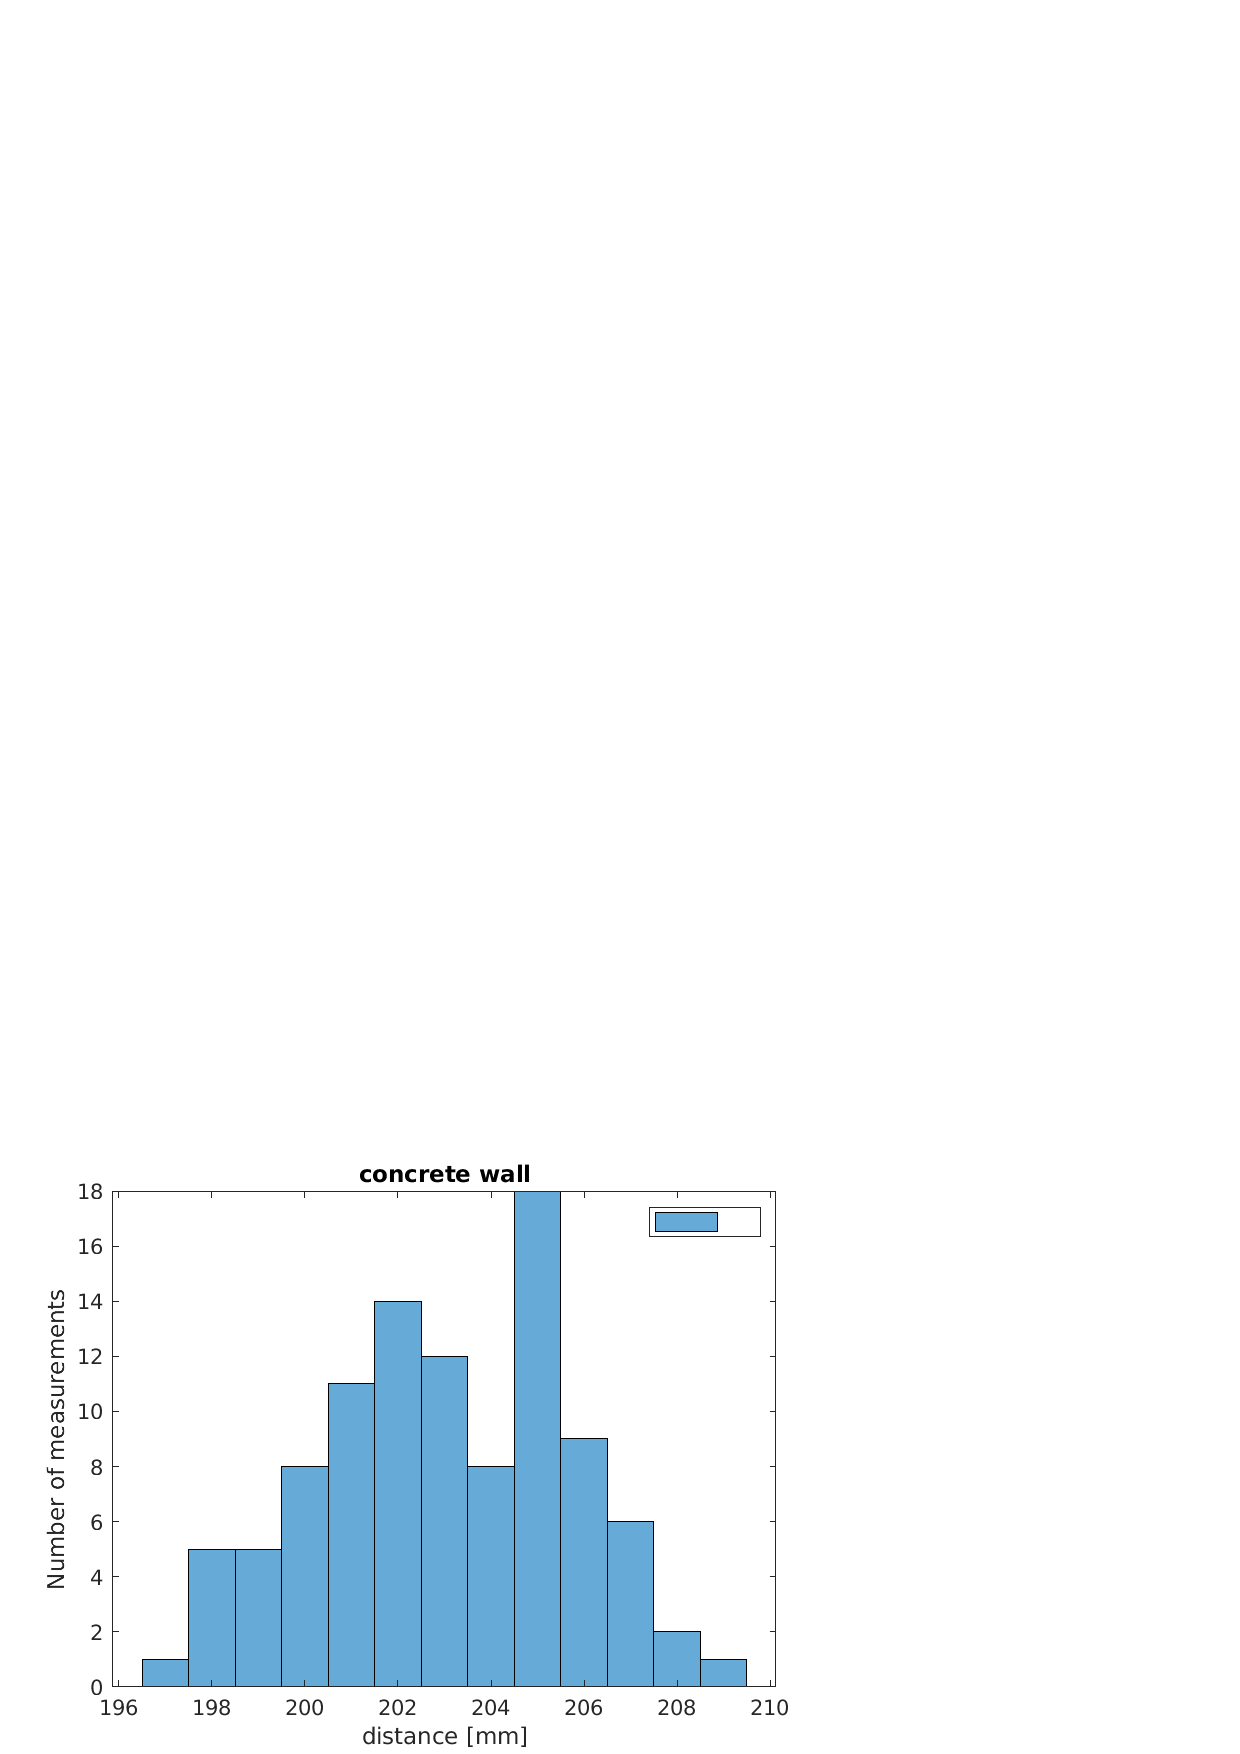
\includegraphics[width=0.9\linewidth]{pictures/concrete_hist.pdf}
		\caption{Ground Truth Distance: $d_{truth}= \unit[200]{mm}$, Standard Error: $\sigma=\unit[2.03]{mm}$, Expected Value: $E=\unit[203]{mm}$}
		\label{fig:surface_hist_con}
\end{figure}
\begin{figure}
		\centering
		\includegraphics[width=0.9\linewidth]{pictures/wooden_wall.pdf}
		\caption{Ground Truth Distance: $d_{truth}= \unit[200]{mm}$, Standard Error: $\sigma=\unit[2.67]{mm}$, Expected Value: $E=\unit[197.06]{mm}$}
		\label{fig:surface_hist_wood}
\end{figure}
\begin{figure}
		\centering
		\includegraphics[width=0.9\linewidth]{pictures/white_wall.pdf}
		\caption{Ground Truth Distance: $d_{truth}= \unit[200]{mm}$, Standard Error: $\sigma=\unit[2.01]{mm}$, Expected Value: $E=\unit[198.01]{mm}$}
		\label{fig:surface_hist_white}
\end{figure}
\begin{figure}
	\centering
	\includegraphics[width=0.9\linewidth]{pictures/plot_angles_90.pdf}
	\caption{Ground Truth Distance: $d_{truth}= \unit[200]{mm}$, Standard Error: $\sigma=\unit[2.03]{mm}$, Expected Value: $E=\unit[198.31]{mm}$, Relative angle: 90°}
	\label{fig:angle90}
\end{figure}
\begin{figure}
	\centering
	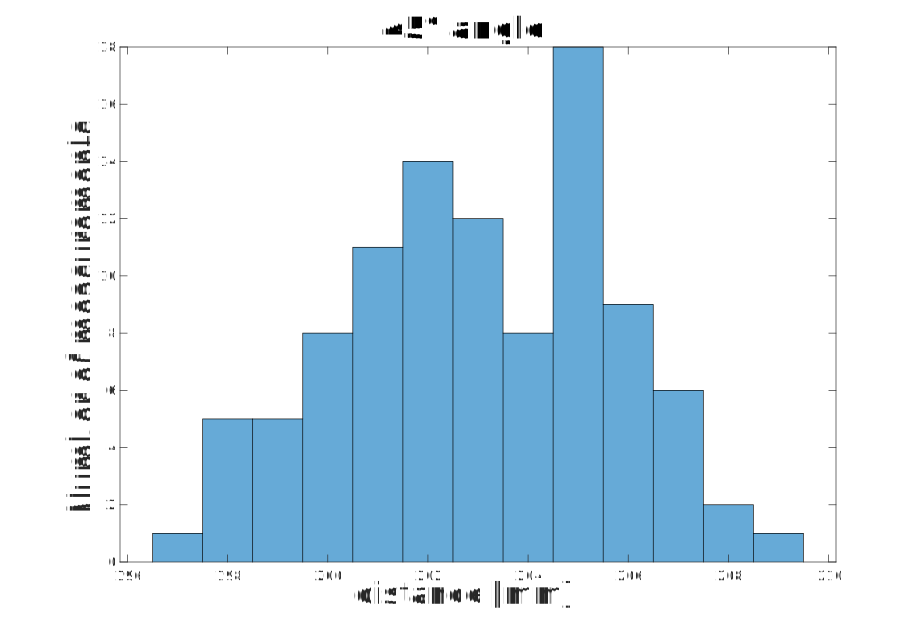
\includegraphics[width=0.9\linewidth]{pictures/plot_angles_45.pdf}
	\caption{Ground Truth Distance: $d_{truth}= \unit[200]{mm}$, Standard Error: $\sigma=\unit[2.69]{mm}$, Expected Value: $E=\unit[203.00]{mm}$, Relative angle: 45°}
	\label{fig:angle45}
\end{figure}
\begin{figure}
	\centering
	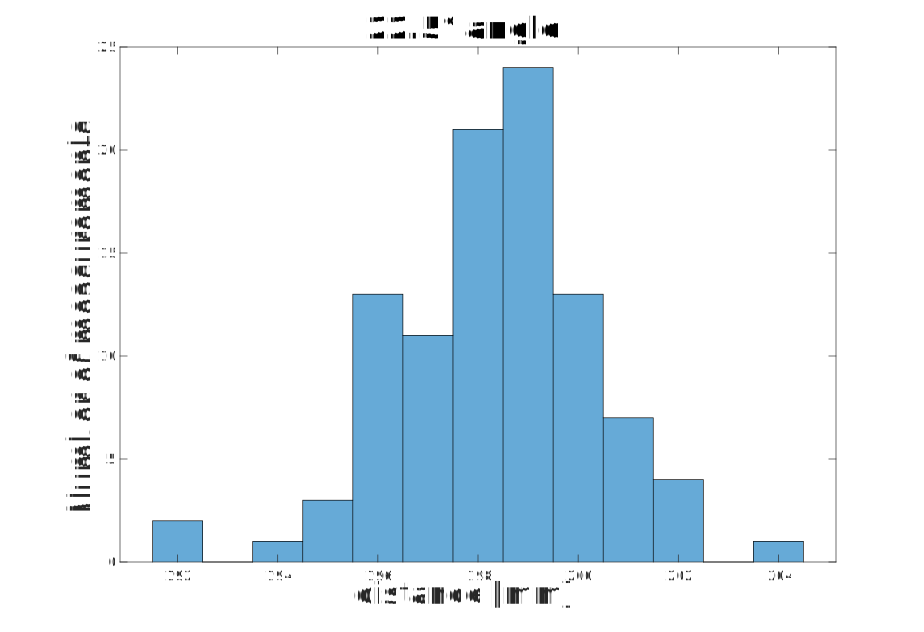
\includegraphics[width=0.9\linewidth]{pictures/plot_angles_22.pdf}
	\caption{Ground Truth Distance $d_{truth}= \unit[200]{mm}$, Standard Error: $\sigma=\unit[3.28]{mm}$, expected Value: $E=\unit[201.62]{mm}$, Relative angle: 22.5°}
	\label{fig:angle22.5}
\end{figure}

\begin{figure}
	\centering
	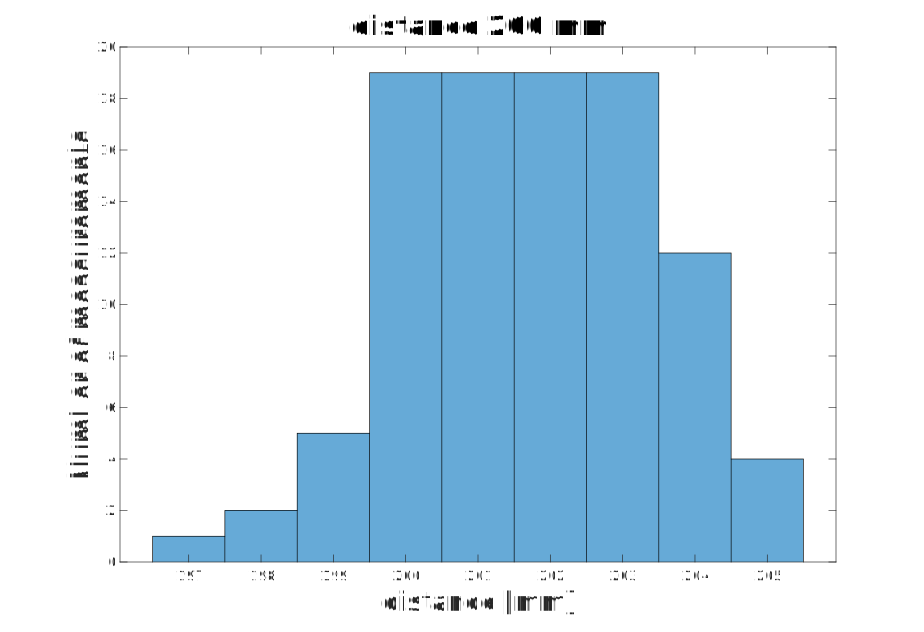
\includegraphics[width=0.9\linewidth]{pictures/plot_dist200.pdf}
	\caption{Ground Truth Distance $d_{truth}= \unit[200]{mm}$, Standard Error: $\sigma=\unit[1.72]{mm}$, Expected Value: $E=\unit[201.70]{mm}$, Relative angle: 90°}
	\label{fig:dist200}
\end{figure}

\begin{figure}
	\centering
	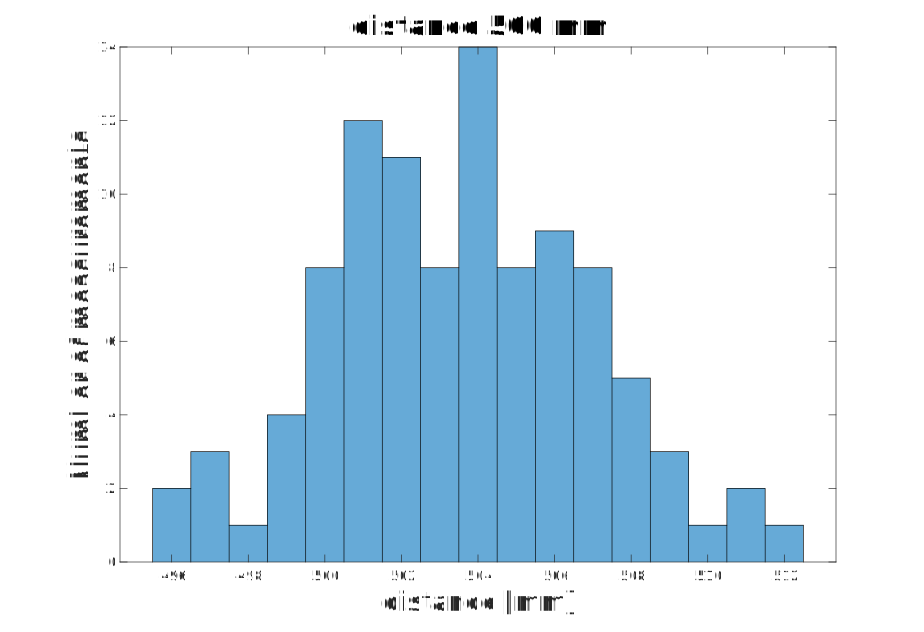
\includegraphics[width=0.9\linewidth]{pictures/plot_dist500.pdf}
	\caption{Ground Truth Distance $d_{truth}= \unit[500]{mm}$, Standard Error: $\sigma=\unit[3.40]{mm}$, Expected Value: $E=\unit[503.52]{mm}$, Relative angle: 90°}
	\label{fig:dist500}
\end{figure}

\begin{figure}
	\centering
	\includegraphics[width=0.9\linewidth]{pictures/plot_dist1000.pdf}
	\caption{Ground Truth Distance $d_{truth}= \unit[1000]{mm}$, Standard Error: $\sigma=\unit[7.01]{mm}$, Expected Value: $E=\unit[1001.6]{mm}$, Relative angle: 90°}
	\label{fig:dist1000}
\end{figure}
The previous testing were all conducted inside, i.e, without a IR source. In the following, the results from measurements outside on a sunny day are presented. First we conducted the measurement in the shadow (\cref{fig:meas_out_shadow}) and second with direct sunlight facing the VL53L0X (\cref{fig:meas_out_sun}). The accuracy of the VL53L0X sensor worsens drastically with a IR source interfering the ranging measurements. To increase the convergence of the sensor we filtered the ranging data with \cref{alg:filter}. The filter evidently improves the data. A convergence toward the ground truth value can be observed (\crefrange{fig:meas_out_shadow filter}{fig:meas_out_sun filter})
\begin{figure}
	\centering
	\includegraphics[width=0.9\linewidth]{pictures/plot_out_shadow.pdf}
	\caption{Measurement outside without direct sunlight. On the x axis is the measurement count and on the y-axis the distance from the sensor to the target. All measurements above 8000 failed due disturbance of the IR in the sunlight. Only 82 out of 100 measurements can be used for further processing. The ground truth distance is $d_{truth}=\unit[200]{mm}$, the expected value is $E=\unit[189.95]{mm}$ and the standard error is $\sigma=\unit[27.51]{mm}$ without considering the failed data points.}
	\label{fig:meas_out_shadow}
\end{figure}

\begin{figure}
	\centering
	\includegraphics[width=0.9\linewidth]{pictures/plot_meas_out.pdf}
	\caption{Measurement outside with direct sunlight. On the x axis is the measurement count and on the y-axis the distance from the sensor to the target. All measurements above 8000 are corrupted due to the IR in the sunlight. Only 18 out of 100 measurements can be used for further processing. The ground truth distance is $d_{truth}=\unit[500]{mm}$, the expected value is $E=\unit[434.54]{mm}$ and the standard error is $\sigma=\unit[98.22]{mm}$ without considering the failed data points.}
	\label{fig:meas_out_sun}
\end{figure}

\begin{figure}
	\centering
	\includegraphics[width=0.9\linewidth]{pictures/plot_filter_shadow.pdf}
	\caption{Comparison of raw data and filtered data (\cref{alg:filter}). On the x axis is the measurement count and on the y-axis the distance from the sensor to the target. Measurement are conducted outside without direct sunlight. The last value of the filtered data is \unit[201.28]{mm} and the ground truth distance is $d_{truth}=\unit[200]{mm}$. A convergence of the filtered data towards the ground truth distance can be observed}
	\label{fig:meas_out_shadow filter}
\end{figure}
\begin{figure}
	\centering
	\includegraphics[width=0.9\linewidth]{pictures/plot_filter_sun.pdf}
	\caption{Comparison of raw data and filtered data (\cref{alg:filter}). On the x axis is the measurement count and on the y-axis the distance from the sensor to the target. Measurement are conducted outside with direct sunlight. The last value of the filtered data is \unit[510.53]{mm} and the ground truth distance is $d_{truth}=\unit[500]{mm}$. A convergence of the filtered data towards the ground truth distance can be observed}
	\label{fig:meas_out_sun filter}
\end{figure}
\section{Avoidance System}
\label{sec:avoidance}
By holding the drone by hands, approaching a wall and receding from it, we were able to make the first measurements and see how the potential field reacts (\cref{fig:pf}). The potential field is implemented according to \cref{eq:angle sp} and computed online. For the parameters we set for the gain $k_{corr}=800000000$ and for the distance of influence $\rho_0=\unit[1500]{mm}$. Additionally, we have added an upper threshold to the corrective angle $\Omega_{corr,thresh}=\unit[\pm1.5]{rad}$. The update rate of the potential field is around \unit[200]{ms}. The potential field behaved as expected. The corrective angle increased exponentially as we approached the wall and decreased as we receded from the wall.\\
\begin{figure}
	\centering
	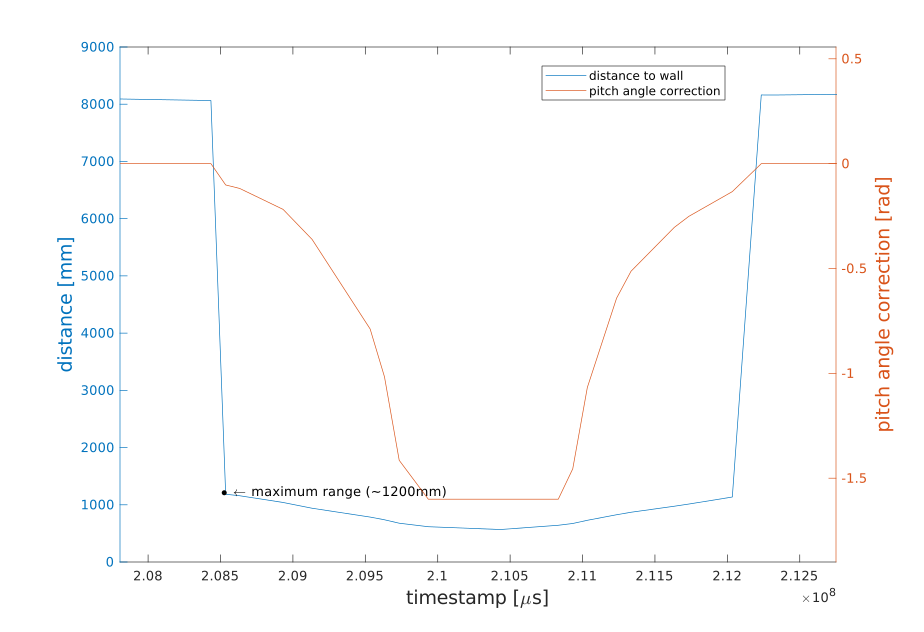
\includegraphics[width=0.9\linewidth]{pictures/plot_pf.pdf}
	\caption{The distance (blue) and corrective pitch angle (orange) are plotted. The VL53L0X starts to detect the wall at a distance of \unit[1200]{mm}. At this distance the potential field start to correct the attitude. The corrective angle increases exponentially as the distance between target and platform decreases. At around \unit[600]{mm} the corrective angle threshold of \unit[-1.5]{rad} is reached. After the reversal point, the corrective angle decreases exponentially.}
	\label{fig:pf}
\end{figure}
As a next step, we manoeuvred the platform towards a wall with a remote control (\cref{fig:maneuvre}). We logged the attitude, the corrective angles, the attitude setpoint from the remote control and the distance between platform and wall (\cref{fig:pf test}). Approaching the wall, the potential field computed the corrective angles correctly forcing the MAV away from the wall. If the manoeuvre is rather aggressive the pilot needs to counter steer the corrective pitch.
\begin{figure}
	\centering
	\includegraphics[width=0.9\linewidth]{pictures/av1.png}
	\includegraphics[width=0.9\linewidth]{pictures/av2.png}
	\includegraphics[width=0.9\linewidth]{pictures/av3.png}
	\includegraphics[width=0.9\linewidth]{pictures/av4.png}
	\includegraphics[width=0.9\linewidth]{pictures/av5.png}
	\includegraphics[width=0.9\linewidth]{pictures/av6.png}
	\includegraphics[width=0.9\linewidth]{pictures/av7.png}	
	\caption{MAV flying towards a wall and autonomously being pushed away by the potential field.}
	\label{fig:maneuvre}
\end{figure}

\begin{figure}
	\centering
	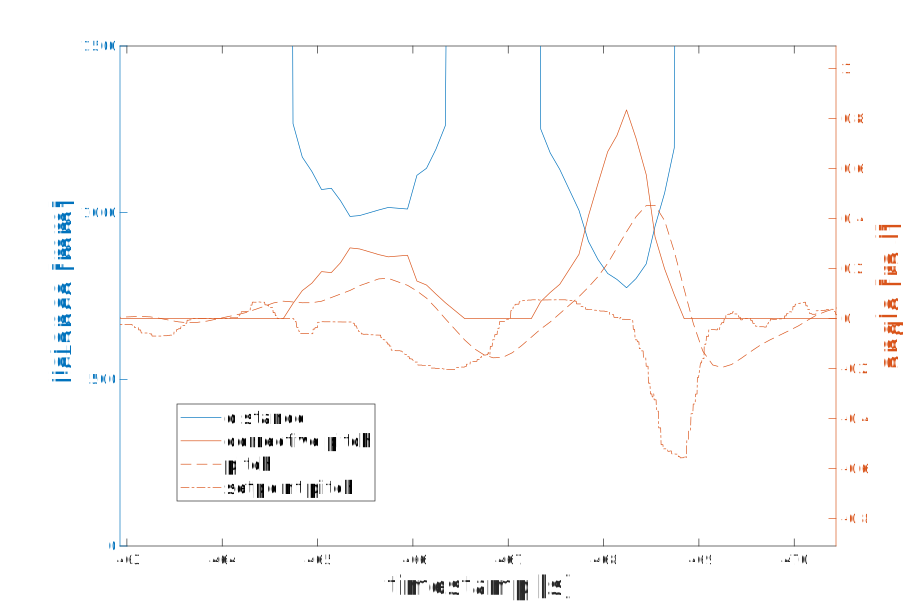
\includegraphics[width=0.9\linewidth]{pictures/plot_pf_test.pdf}
	\caption{The distance between platform and wall, corrective pitch angle computed by the potential field, pitch of the platform and pitch set-point of the remote control are plotted. The VL53L0X ranging sensors have a maximum range of \unit[1200]{mm} thus the distance measurement less and equal to \unit[1200]{mm} are valid. Two approaches of the platform towards the wall can be observed. The first one is rather slow which results in a gentle repulsive force. The second approach is more aggressive followed by a fast change of the corrective pitch. This leads to a fast change in pitch what destabilizes the platform.    Consequently, the pilot has to manually counter steer the corrective pitch.}
	\label{fig:pf test}
\end{figure}


